\section{Design}
TODO:
We use an agent for this target group

In order to measure the enjoyability of a LBG with a game activity as the navigational method between POIs, we developed a location-based game (LBG). The game takes place in Aalborg, Denmark and the points of interest (POIs) are three street art paintings\cite{streetart}. The game makes players walk between the three POIs on a route with a total length of 1.8km (see Figure \ref{FinalRoute}). Due to requirements from the method of the experiment as described in (INSERT REFERENCE TO METHOD SECTION), the particular route was chosen on the basis of it having a close to equal amount of intersections in the road between POIs as well as a close to equal distance between the POIs. In the process of designing the navigational game activity, four initial designs were created as paper prototypes and one was chosen to be used in the game on the basis of three initial tests of the designs. The participants of each test were a child in the age group of 8-11 years and the child's parent.

\begin{figure}[hbtp]
\centering
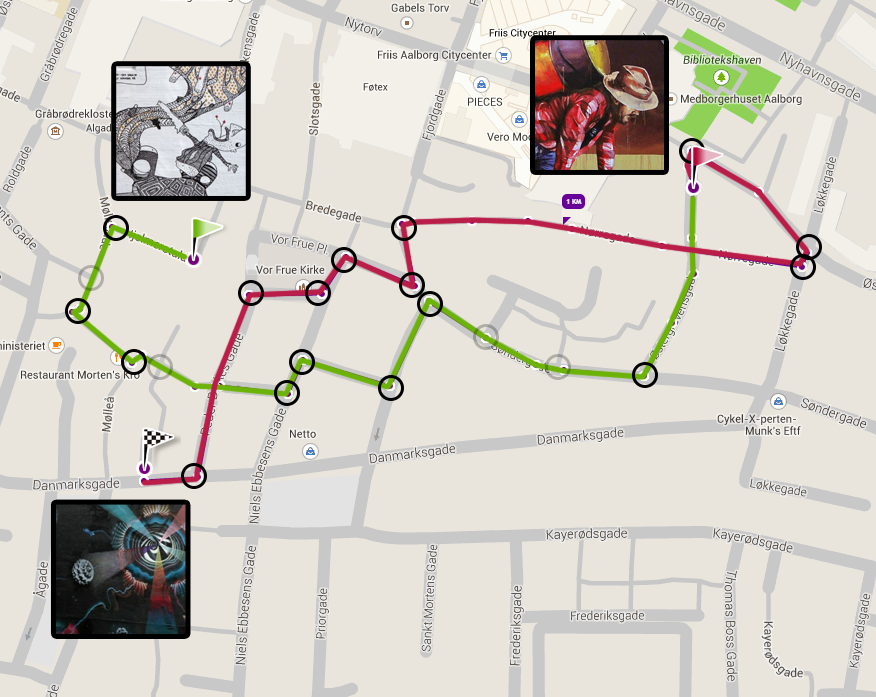
\includegraphics[scale=0.3]{Pics/FinalRoute.png}
\caption{The route between the three street art paintings.}
\label{FinalRoute}
\end{figure}

\subsection{Choice of Navigational Game Activity}
When designing the four navigational game activities, inspiration was taken from game activities that take place at POIs in other LBGs as well as popular children's games, since they are familiar to most children, causing a lower learning curve. As mentioned earlier, Team Exploration\cite{GamingOnTheMove} is a game where players match pictures in the virtual space to the environment in the physical space and progress in the game by specifying which pictures belong to certain areas. This game activity can be related to the game 

Mention landmarks in navigation section!

 , where players  and CityTreasure\cite{botturi2009city}. 

\subsection{Lost on Earth}
